\documentclass[10pt,a4paper]{article}
\usepackage[T1]{fontenc}
\usepackage{lmodern,microtype}
\usepackage[margin=23mm]{geometry}
\usepackage{amsmath,amssymb,graphicx,booktabs,tabularx,longtable,array}
\usepackage[table]{xcolor}
\usepackage{enumitem,float,caption,xurl,listings,circuitikz}
\usepackage[numbers,sort&compress]{natbib}
\usepackage[colorlinks=true,allcolors=blue!50!black]{hyperref}
\usetikzlibrary{positioning,arrows.meta,shapes.geometric}
\setlist{nosep,leftmargin=*}
\setlength{\parindent}{0pt}
\setlength{\parskip}{6pt}
\widowpenalty=10000\clubpenalty=10000
\renewcommand{\tabularxcolumn}[1]{>{\raggedright\arraybackslash}p{#1}}
\renewcommand{\arraystretch}{1.2}
\captionsetup{font=small,labelfont=bf}
\hypersetup{pdftitle={CrashGuard: Crash Detection and Emergency Alerts},pdfauthor={Adheesh Garg, Ayan Gatani, Aastha Gupta, Syamasudha Veeragandham}}
\bibliographystyle{IEEEtran}
\lstset{basicstyle=\ttfamily\small,breaklines=true,columns=fullflexible,frame=single}
\newcommand{\degree}{\ensuremath{^{\circ}}}

% Robust image loader ensuring zero compile errors in Overleaf even if figures folder is not uploaded
\newcommand{\safeincludegraphics}[2][]{%
  \IfFileExists{#2}{%
    \includegraphics[#1]{#2}%
  }{%
    \IfFileExists{figures/#2}{%
      \includegraphics[#1]{figures/#2}%
    }{%
      \fbox{%
        \parbox{\dimexpr\linewidth-2\fboxsep-2\fboxrule\relax}{%
          \vspace{1.2cm}%
          \centering%
          \texttt{[Figure Graphic: \detokenize{#2}]}\\[6pt]%
          {\footnotesize\normalfont(Upload image file to Overleaf project root or \texttt{figures/} folder to render)}\par%
          \vspace{1.2cm}%
        }%
      }%
    }%
  }%
}
\newcommand{\fig}[3]{\begin{figure}[H]\centering\safeincludegraphics[width=#2\linewidth]{#1}\caption{#3}\end{figure}}

% Embedded experimental macros (self-contained, no external file required)
\newcommand{\SimulationSeed}{20260828}
\newcommand{\SimulationEvents}{675}
\newcommand{\SimulationSamples}{675,000}
\newcommand{\PositiveEvents}{150}
\newcommand{\NegativeEvents}{525}
\newcommand{\CrashGuardSensitivity}{76.0\%}
\newcommand{\CrashGuardSpecificity}{100.0\%}
\newcommand{\CrashGuardFOne}{0.864}
\newcommand{\CrashGuardTP}{114}
\newcommand{\CrashGuardTN}{525}
\newcommand{\CrashGuardFP}{0}
\newcommand{\CrashGuardFN}{36}
\newcommand{\CrashGuardSensitivityLow}{68.6\%}
\newcommand{\CrashGuardSensitivityHigh}{82.1\%}
\newcommand{\CrashGuardSpecificityLow}{99.3\%}
\newcommand{\CrashGuardConfirmationDelayMs}{2315}
\newcommand{\CrashGuardImpactThreshold}{2.00}
\newcommand{\CrashGuardLowImpactThreshold}{0.35}
\newcommand{\CrashGuardRotationThreshold}{90}
\newcommand{\CrashGuardTiltThreshold}{55}
\newcommand{\CrashGuardRestHoldMs}{2000}
\newcommand{\CrashGuardCorrelationMs}{750}
\newcommand{\CrashGuardRideQualificationMs}{1000}
\newcommand{\CrashGuardRideMemoryMs}{5000}
\newcommand{\BaselineSensitivity}{89.3\%}
\newcommand{\BaselineSpecificity}{45.0\%}
\newcommand{\BaselineFOne}{0.468}
\newcommand{\OrderedSensitivity}{26.0\%}
\newcommand{\OrderedSpecificity}{100.0\%}
\newcommand{\OrderedFOne}{0.413}
\newcommand{\OrderedConfirmationDelayMs}{3120}
\newcommand{\BoubezoulSensitivity}{90.0\%}
\newcommand{\BoubezoulSpecificity}{83.0\%}
\newcommand{\BoubezoulFOne}{0.722}
\newcommand{\BoubezoulTP}{135}
\newcommand{\BoubezoulTN}{436}
\newcommand{\BoubezoulFP}{89}
\newcommand{\BoubezoulFN}{15}
\newcommand{\BoubezoulConfirmationDelayMs}{2280}
\newcommand{\McNemarBoubezoulStat}{40.81}
\newcommand{\McNemarBoubezoulPValue}{1.6785e-10}
\newcommand{\McNemarOrderedStat}{73.01}
\newcommand{\McNemarOrderedPValue}{0.0000e+00}
\newcommand{\McNemarBaselineStat}{232.44}
\newcommand{\McNemarBaselinePValue}{0.0000e+00}
\newcommand{\ExternalFallCount}{4}
\newcommand{\ExternalManoeuvreCount}{7}
\newcommand{\ExternalFourGPass}{0}
\newcommand{\ExternalTwoHundredPass}{0}
\newcommand{\ExternalCrashGuardImpactPass}{4}
\newcommand{\ExternalCrashGuardRotationPass}{4}

% Embedded bibliography database for direct, one-file Overleaf copy-paste
\begin{filecontents*}[overwrite]{\jobname.bib}
@article{tian2026transformer,
  author  = {Jingxiao Tian and Shengjie Xu and Peter Gerstoft and Mahasweta Sarkar and Alison A. Moore and Patrick Mercier and Christopher Paolini},
  title   = {A Multi-Head Attention Transformer Model for Wearable in Situ Fall Detection},
  journal = {IEEE Access},
  volume  = {14},
  pages   = {85242--85262},
  year    = {2026},
  doi     = {10.1109/ACCESS.2026.3697249}
}
@article{boubezoul2013algorithm,
  author  = {Abderrahmane Boubezoul and St{\'e}phane Espi{\'e} and Bruno Larnaudie and Samir Bouaziz},
  title   = {A Simple Fall Detection Algorithm for Powered Two Wheelers},
  journal = {Control Engineering Practice},
  volume  = {21},
  number  = {3},
  pages   = {286--297},
  year    = {2013},
  doi     = {10.1016/j.conengprac.2012.10.009}
}
@article{boubezoul2019dataset,
  author  = {Abderrahmane Boubezoul and Fabien Dufour and Samir Bouaziz and Bruno Larnaudie and St{\'e}phane Espi{\'e}},
  title   = {Dataset on Powered Two Wheelers Fall and Critical Events Detection},
  journal = {Data in Brief},
  volume  = {23},
  pages   = {103828},
  year    = {2019},
  doi     = {10.1016/j.dib.2019.103828}
}
@article{gelmini2021novel,
  author  = {Simone Gelmini and Silvia C. Strada and Mara Tanelli and Sergio M. Savaresi and Claudio De Tommasi},
  title   = {A Novel Crash Detection Algorithm for Two-Wheeled Vehicles},
  journal = {IEEE Transactions on Intelligent Vehicles},
  volume  = {6},
  number  = {1},
  pages   = {88--99},
  year    = {2021},
  doi     = {10.1109/TIV.2020.3028462}
}
@misc{blynktemplate,
  author = {{Blynk}},
  title  = {Device Template Documentation},
  year   = {2026},
  url    = {https://docs.blynk.io/en/concepts/device-template},
  note   = {Accessed 11 September 2026}
}
@misc{blynkdata,
  author = {{Blynk}},
  title  = {Send Data From Hardware to Blynk},
  year   = {2026},
  url    = {https://docs.blynk.io/en/getting-started/how-to-display-any-sensor-data-in-blynk-app},
  note   = {Accessed 11 September 2026}
}
@misc{blynkevents,
  author = {{Blynk}},
  title  = {Log Event: Firmware API},
  year   = {2026},
  url    = {https://docs.blynk.io/en/blynk-library-firmware-api/log-event},
  note   = {Accessed 11 September 2026}
}
@misc{wokwiscenarios,
  author = {{Wokwi}},
  title  = {Automation Scenarios},
  year   = {2026},
  url    = {https://docs.wokwi.com/wokwi-ci/automation-scenarios},
  note   = {Accessed 11 September 2026}
}
@misc{wokwiwifi,
  author = {{Wokwi}},
  title  = {{ESP32 WiFi Networking}},
  year   = {2026},
  url    = {https://docs.wokwi.com/guides/esp32-wifi},
  note   = {Accessed 11 September 2026}
}
@manual{mpu6050datasheet,
  author       = {{TDK InvenSense}},
  title        = {{MPU-6000 and MPU-6050 Product Specification}, Revision 3.4},
  year         = {2013},
  url          = {https://invensense.tdk.com/wp-content/uploads/2015/02/MPU-6000-Datasheet.pdf}
}
@manual{esp32datasheet,
  author       = {{Espressif Systems}},
  title        = {{ESP32 Series Datasheet}, Version 5.3},
  year         = {2026},
  url          = {https://www.espressif.com/sites/default/files/documentation/esp32_datasheet_en.pdf}
}
@article{wilson1927interval,
  author  = {Edwin B. Wilson},
  title   = {Probable Inference, the Law of Succession, and Statistical Inference},
  journal = {Journal of the American Statistical Association},
  volume  = {22},
  number  = {158},
  pages   = {209--212},
  year    = {1927},
  doi     = {10.1080/01621459.1927.10502953}
}
@article{sisfall,
 author={Angela Sucerquia and José López and Jesús Vargas-Bonilla},
 title={SisFall: A Fall and Movement Dataset},
 journal={Sensors},
 year={2017},
 doi={10.3390/s17010198}
}
@article{survey,
 author={Eduardo Casilari and José-Antonio Santoyo-Ramón and José-Manuel Cano-García},
 title={Analysis of Public Datasets for Wearable Fall Detection Systems},
 journal={Sensors},
 year={2017},
 doi={10.3390/s17071513}
}
@article{cnn,
 author={Eduardo Casilari and Raúl Lora-Rivera and Francisco García-Lagos},
 title={A Study on the Application of Convolutional Neural Networks to Fall Detection Evaluated with Multiple Public Datasets},
 journal={Sensors},
 year={2020},
 doi={10.3390/s20051466}
}
@article{kfall,
 author={Xiaoqun Yu and Jaehyuk Jang and Shuping Xiong},
 title={A Large-Scale Open Motion Dataset (KFall) and Benchmark Algorithms for Detecting Pre-impact Fall of the Elderly Using Wearable Inertial Sensors},
 journal={Frontiers in Aging Neuroscience},
 year={2021},
 doi={10.3389/fnagi.2021.692865}
}
@misc{musci, author={Mirto Musci and Daniele De Martini and Nicola Blago and Tullio Facchinetti and Marco Piastra}, title={Online Fall Detection using Recurrent Neural Networks}, year={2018}, doi={10.48550/arXiv.1804.04976}, url={https://arxiv.org/abs/1804.04976}}
@misc{localcode, author={{CrashGuard project}}, title={Shared Detector, Firmware, Dataset Generator and Firmware Experiment Harness}, year={2026}, note={Reproducible source distributed with this report; see Data Availability and the repository README}}
@article{ecall2025,
 author={Jessica Leoni and Simone Gelmini and Giulio Panzani and Mara Tanelli and Sergio Matteo Savaresi},
 title={Automatic eCall in Powered Two-Wheelers: A Dynamics-Based Approach},
 journal={IEEE Transactions on Intelligent Transportation Systems},
 year={2025},
 doi={10.1109/tits.2025.3545907},
 url={https://doi.org/10.1109/tits.2025.3545907},
 volume={26},
 pages={4365-4379}
}
@article{dual2026,
 author={Abheek Pradhan and Sana Alamgeer and Rakesh Suvvari and Syed Tousiful Haque and Anne H. H. Ngu},
 title={Dual-Stream Transformer with Kalman-Based Sensor Fusion for Wearable Fall Detection},
 journal={Big Data and Cognitive Computing},
 year={2026},
 doi={10.3390/bdcc10030090},
 url={https://doi.org/10.3390/bdcc10030090},
 volume={10},
 pages={90}
}
@misc{rodegast2024, author={Philipp Rodegast and Steffen Maier and Jonas Kneifl and J{\"o}rg Fehr}, title={On using Machine Learning Algorithms for Motorcycle Collision Detection}, year={2024}, doi={10.48550/arXiv.2403.09491}, url={https://arxiv.org/abs/2403.09491}}
@article{mcnemar1947,
 author={Quinn McNemar},
 title={Note on the sampling error of the difference between correlated proportions or percentages},
 journal={Psychometrika},
 volume={12},
 number={2},
 pages={153--157},
 year={1947},
 doi={10.1007/BF02295996}
}
\end{filecontents*}
\begin{document}
\begin{center}
{\LARGE\bfseries CrashGuard: Simulation-Based Evaluation of an IoT Crash Detection and Emergency Alert System for Two-Wheeler Riders\par}
\vspace{6mm}
Adheesh Garg\textsuperscript{1}, Ayan Gatani\textsuperscript{1}, Aastha Gupta\textsuperscript{1},\\
Syamasudha Veeragandham\textsuperscript{2,*}\\[3mm]
\textsuperscript{1,2}School of Computer Science and Engineering,\\
Vellore Institute of Technology, Vellore, Tamil Nadu, India -- 632014\\[3mm]
{\small\href{mailto:adheesh.garg2023@vitstudent.ac.in}{adheesh.garg2023@vitstudent.ac.in}\\
\href{mailto:ayan.gatani2023@vitstudent.ac.in}{ayan.gatani2023@vitstudent.ac.in}\\
\href{mailto:aastha.gupta2023@vitstudent.ac.in}{aastha.gupta2023@vitstudent.ac.in}\\
\textsuperscript{*}Corresponding author: \href{mailto:syamasudha.v@vit.ac.in}{syamasudha.v@vit.ac.in}}\\[3mm]
\end{center}
\begin{abstract}
We present CrashGuard, a low-cost handlebar device which detects a motorcycle crash and sends out an emergency alert, and we evaluate it by simulation alone. An ESP32 microcontroller reads a six-axis inertial sensor at 100 Hz, and the decision is taken by a small finite-state machine. For a crash to be confirmed four things must happen, in this order. The motorcycle must have been ridden; there must be an impact or a sudden unloading; a strong rotation must follow shortly afterwards; and the motorcycle must then lie tilted and still for two seconds. The device then turns on a light and a buzzer and gives the rider 15 seconds to cancel, after which a single event goes to a cloud service. We did not build a physical prototype. The results come from generated motion data, from a public motorcycle dataset and from the unchanged firmware, which we ran against simulated peripherals.

On a fresh set of 270 generated events CrashGuard rejected all 210 non-crash events and caught every one of the 30 high-side crashes. It missed, however, 17 of the 30 low-side crashes, which puts its overall sensitivity at 71.7\% (F1 = 0.835). On the same events we also ran a rule built on the staged structure of the motorcycle fall detector of Boubezoul et al.\ (2013). This rule detected more crashes (86.7\%) but gave 34 false alarms, and by McNemar's test the two rules differ significantly ($\chi^2 = 13.40$, $p = 0.00025$). The tilt, rotation and rest-hold thresholds were swept one parameter at a time. From the sweeps it appears that the 2 s rest hold is what suppresses the nuisance alarms, and that a lower rotation gate could win back some of the missed low-side crashes (the latter is still to be confirmed on separate data). Fourteen firmware tests exposed three defects. The rest timer keeps running when sensor reads are missing, a failed cloud connection holds up the main loop for 5 s, and an alert which falls due during a Wi-Fi outage is never retried. With a simple battery model the device lasts 12.64 hours at a 120 mA, 5 V load. Code, data and scripts are released, so every experiment reported here can be repeated.
\end{abstract}
\noindent\textbf{Keywords:} IoT; ESP32; MPU6050; Motorcycles; Detection; Simulation; Alerts; Safety.
\clearpage

\section{Introduction}
A motorcyclist who comes off the bike on an empty road can lie there unnoticed for quite some time. A device on the motorcycle which recognises the crash and calls for help would shorten this delay, but only if it does not raise false alarms so often that the rider switches it off. So the task is a detection problem with two kinds of error, and the two kinds do not cost the same. A missed crash may leave an injured rider without help. One false alarm costs little, but many of them make the device useless. In this paper we describe and evaluate CrashGuard, a prototype mounted on the handlebar and built around an ESP32 microcontroller and an MPU-6050 inertial sensor. We should say at once that no physical hardware was assembled. The evaluation relies on generated motion data, on public motorcycle recordings and on the real firmware run against simulated peripherals. In the rest of this section we go through the earlier work which shaped the design, one paper at a time.

Boubezoul et al.~\cite{boubezoul2013algorithm} were among the first to look at fall detection for powered two-wheelers (PTWs) as a problem of its own. Their main point is that a single threshold on acceleration is unreliable, as a motorcycle leans in ordinary riding and the road surface sends shocks through it. They detect a fall in stages; first the start of the fall, then the growth of the lean angle, and then a period of rest afterwards. CrashGuard keeps this staged view. Since it has to run on an inexpensive handlebar unit, the stages are written as a small finite-state machine, with a ride-qualification step put in front of them and a cancellation window behind. We compare our detector with a rule following the structure of their algorithm, and with two simpler rules, all on exactly the same six-axis data.

A few years later the same group published recordings of real PTW falls and critical manoeuvres~\cite{boubezoul2019dataset}. Such data are rare, crashing a motorcycle on purpose being both expensive and dangerous. The falls serve as positive examples. The manoeuvres (hard braking, accelerating in a curve, a badly degraded track and so on) are negative examples, and they test whether a detector can keep quiet. We take four falls and seven manoeuvres from this set and use them for a limited purpose only, namely to check whether the signals cross the acceleration and rotation gates of CrashGuard. In other words we test the scale of our thresholds, not the full decision. All four falls cross both gates. The unit conversion, the filtering and the choice of time windows are published with the code.

Gelmini et al.~\cite{gelmini2021novel} developed a crash detection algorithm for two-wheeled vehicles and tested it on experimental riding data. For us their work is mostly a lesson about coverage. Ordinary riding produces signals of many kinds, and a detector which has seen only a few convenient crash examples tells us little about how it will behave on the road. For this reason our simulated data contain braking, sharp turns, potholes, speed breakers, an impact followed by recovery and a parked motorcycle tipping over, besides two kinds of crash. Low-side and high-side crashes are kept as separate classes. This turns out to matter. In the fresh data every high-side crash is detected and all 17 misses are low-side crashes.

On the side of human falls, Sucerquia et al.~\cite{sisfall} introduced SisFall, a dataset recorded with a device worn at the waist. Its signals come from a human body and not from a handlebar, so we do not use them. What we take from it is the design. It contains many everyday activities which are not falls, and a detector evaluated on it has to show that it stays quiet, not only that it fires. We follow the same principle; seven of our nine scenario classes are negative, and the class counts are given with every result. On the fresh events CrashGuard rejects all 210 negatives, though of course this holds only within our signal model.

Casilari et al.~\cite{survey} compared the public datasets for wearable fall detection and found that they differ a good deal in sensor position, sampling rate, recorded activities and recording protocol. A sensitivity of, say, 95\% measured on one dataset may tell little about another. The practical consequence for a new study is that the data have to be described well enough for a reader to judge what the numbers mean. We therefore report the channel units, the sampling rate, the random seeds, the noise and bias levels, the clipping limits and the kinematic transformation used by the generator. No event is ever split between the development, validation and test subsets, and we use a second random stream to check that the results repeat.

In a later study Casilari et al.~\cite{cnn} trained convolutional networks on several public fall datasets and showed that the outcome depends strongly on the repository used. This made us careful about what our own second dataset can show. A new random seed gives new events, but these come from the same generator, the same mounting position and the same model of the motorcycle. We call the result a fresh-seed evaluation, and claim nothing more for it. The public PTW recordings give evidence of another kind (about the physical scale of the signals), and the two are reported in separate tables. A stronger test, with whole vehicles or riding sessions held out, is left for future work.

Musci et al.~\cite{musci} used recurrent neural networks (LSTMs) for online fall detection on an annotated version of SisFall. Their model reads a sequence of samples rather than one sample at a time, and we agree that most of the information lies in the order of events in time. We just encode it in a different way. In place of a learned model we have explicit timing rules, namely a correlation window between impact and rotation, a verification timeout and a hold time for the rest condition. One advantage of explicit rules is that the offline replay and the firmware run the same C++ code, so the two cannot disagree. Another is that when a fault is injected, the transition at which the behaviour went wrong can be read straight off the log.

Yu et al.~\cite{kfall} published KFall, a large dataset with temporal labels, meant for pre-impact fall detection. A pre-impact detector (for example one which triggers a wearable airbag) has to act within a fraction of a second. Our device acts after the event and has a few seconds to spare. The two problems thus need different timing measures, and it matters where a delay measurement starts and where it stops. We measure the time from the first candidate sample to confirmation separately from the 15 s cancellation window which comes after it. On the fresh events the median of the former is 2.33 s. The firmware tests check that the deadline at the end of the window is met to the millisecond.

Rodegast et al.~\cite{rodegast2024} trained machine-learning models for motorcycle collision detection on simulated accidents and simulated normal riding. They aim at a passive safety system, which has to fire quickly and must not fire by mistake. We aim at a warning which the rider can cancel. A slower decision is then acceptable, but nuisance alarms are still costly. Like them we rely on simulation. Our data were generated after the detector rules had been fixed, and every rule we compare gets exactly the same events, so the trade-off between missed crashes and false alarms can be read directly from the confusion counts.

Leoni et al.~\cite{ecall2025} proposed an automatic eCall method for motorcycles based on vehicle dynamics. They separate high-side crashes, in which the vehicle rotates fast, from low-side crashes, in which the motorcycle slides out more slowly. This distinction is at the centre of our results. A threshold set for a fast and violent high-side crash may simply not see a slow slide. In our data CrashGuard rejects every non-crash event, but its low-side recall on the fresh set is only 43.3\%, and we consider this the main weakness of the detector. It is reported separately, so that the overall accuracy of 93.7\% is not taken to mean uniform protection.

Tian et al.~\cite{tian2026transformer} used a multi-head attention transformer for fall detection with a sensor worn on the shin. They report a test sensitivity of 90.5\% and an overall accuracy of 93.1\%, and discuss how class imbalance affects numbers of this kind. Their sensor sits on a human leg and ours on a handlebar. The figures are not comparable and we make no attempt to compare them. We cite the work as recent evidence of what learned sequence models can do. We have also taken from it the habit of reporting class counts, F1 and sensitivity next to accuracy; with 210 negatives and only 60 positives, accuracy on its own would flatter our detector.

Finally, Pradhan et al.~\cite{dual2026} combined a dual-stream transformer with Kalman-filter fusion of inertial signals, and report an F1-score of 91.10\% on SmartFallMM in a subject-wise evaluation. Two of their ideas seem worth adopting later on. One is the fusion of complementary inertial signals, the other is holding out whole groups during evaluation (for us these would be vehicles or riding sessions). At present CrashGuard uses three hand-designed features and fixed rules. Its contribution is elsewhere; it is a light decision sequence in which every state can be observed and tested.

\subsection{Research Gaps and Demonstrated Improvements}

\subsubsection*{Identified Research Gaps}
Taken together, the work above leaves three gaps which matter for a small device of the kind we build.
\begin{enumerate}[label=\textbf{Gap \arabic*:}]
\item \textbf{Thresholds on acceleration alone.} A fixed threshold on the acceleration magnitude cannot ignore hard road shocks (potholes, rumble strips, speed breakers) and at the same time detect slow, low-energy slides.
\item \textbf{Overall accuracy hides missed low-side crashes.} If most test events are negative, a high overall accuracy can go together with poor detection of one type of crash, typically the low-side slide with its gentle deceleration.
\item \textbf{The alert chain is rarely tested.} Most studies stop at classifier metrics. They do not test what the device does when the sensor fails, when the rider cancels, when the cloud service does not answer or when the battery runs down.
\end{enumerate}

\subsubsection*{Demonstrated Engineering Contributions}
The staged decision is due to Boubezoul et al.~\cite{boubezoul2013algorithm}. What we contribute concerns its use in a small handlebar device, and the way it is evaluated.
\begin{enumerate}[label=\textbf{\arabic*.}]
\item \textbf{Ride qualification.} A leaky-bucket filter of recent activity. A parked motorcycle which tips over, or a knock while standing, is then not taken for a crash.
\item \textbf{Local warning and cancellation.} A light and a buzzer, and after them a fixed 15 s window for the rider to cancel, before anything is sent.
\item \textbf{Comparison on identical data.} CrashGuard is compared on the same events with a rule following the structure of Boubezoul et al.~\cite{boubezoul2013algorithm} and with two simpler rules, using paired McNemar tests.
\item \textbf{Threshold sweeps.} The tilt, rotation and rest-hold thresholds are varied one at a time over 29 settings. The aim is to see which of them controls the missed low-side crashes and which the false alarms.
\item \textbf{Firmware fault tests.} The unchanged firmware is run against simulated peripherals in 14 scenarios. These exposed three defects, in the rest timer, in a blocking network call and in the missing retry after a network outage.
\end{enumerate}
We repeat that nothing was built or measured in hardware. Every finding comes from simulation, from models of virtual peripherals or from public recordings.

\subsection{Research Objectives}
\begin{enumerate}
\item To implement and evaluate a 100 Hz six-axis state machine which detects crash-like events on a motorcycle handlebar, with a local warning which the rider can cancel.
\item To compare CrashGuard with a rule following Boubezoul et al.~\cite{boubezoul2013algorithm} and with two simpler rules, on the primary and on the fresh-seed event sets, and to report confusion counts, sensitivity, specificity, F1, delay and paired McNemar tests.
\item To find out, by sweeping the rest-tilt, rotation and rest-hold thresholds, how each of them affects low-side recall and false alarms.
\item To run the firmware with controlled virtual peripherals under sensor, calibration, timing and communication faults, and to record both the expected and the actual behaviour.
\item To publish the data, plots, circuit and architecture diagrams and the power model, along with a plain account of the limitations.
\end{enumerate}

\section{Related Work}
Here the same sources are grouped by topic, and for each we say briefly what it does. How each of them affects our design was explained already in the introduction.

\textbf{Motorcycle fall and crash detection.} Boubezoul et al.~\cite{boubezoul2013algorithm} gave a simple fall detection algorithm for PTWs, which recognises a fall in stages from the motion of the vehicle. Later the same group released recordings of PTW falls and critical manoeuvres~\cite{boubezoul2019dataset}, and we use these for an external check of the signal scale. Gelmini et al.~\cite{gelmini2021novel} studied crash detection for two-wheeled vehicles on experimental riding data, and stressed how varied ordinary riding is. Rodegast et al.~\cite{rodegast2024} trained classifiers on simulated motorcycle collisions, for fast activation of passive safety systems. Leoni et al.~\cite{ecall2025} gave a dynamics-based eCall method which treats fast high-side motion and slower side slips differently.

\textbf{Human fall detection and its datasets.} SisFall~\cite{sisfall} contains waist-worn recordings of falls and of activities of daily living. Casilari et al.~\cite{survey} compared public datasets of this kind and showed how much they differ in sensor position, sampling and protocol; in a later study~\cite{cnn} they found that the results of convolutional networks depend on the dataset used. KFall~\cite{kfall} added synchronised temporal labels and benchmark algorithms for pre-impact detection.

\textbf{Learned sequence models.} Musci et al.~\cite{musci} applied LSTM networks to online fall detection on an annotated version of SisFall. Tian et al.~\cite{tian2026transformer} used a multi-head attention transformer for a device mounted on the shin, and report 90.5\% test sensitivity and 93.1\% accuracy after class balancing and focal-loss training. Pradhan et al.~\cite{dual2026} combined a dual-stream transformer with Kalman-based fusion and report 91.10\% F1 in a 21-fold leave-one-subject-out evaluation on SmartFallMM. Mountings, labels and populations in these studies are not the same as ours, so their numbers serve as context and not as a ranking.

\textbf{The cloud interface.} The Blynk documentation on device templates and on event logging~\cite{blynktemplate,blynkevents} defines the device identity, the event code and the firmware call we use for reporting an incident. This is not detection research. It does, however, fix the boundary between the controller and the cloud, and our firmware tests record what happens at that boundary when an event is sent, when it is skipped and when the connection times out.

The sources are collected in Table~\ref{tab:prior}. For each one the table gives the sensing domain or method, and says which part of our design or evaluation it informs. The rows describe how the sources relate to our work. They do not rank methods on a common dataset.

\small
\begin{longtable}{|>{\raggedright\arraybackslash}p{.19\linewidth}|>{\raggedright\arraybackslash}p{.23\linewidth}|>{\raggedright\arraybackslash}p{.49\linewidth}|}
\caption{Prior work on motorcycle crashes, human falls, datasets and the IoT interface, and the role of each in CrashGuard. The first column names the source, the second its sensing domain or method, and the third the design or evaluation decision it informs. The public motorcycle data are an external signal reference. The human-fall studies inform how we evaluate, but they use other mounting positions and other labels.}\label{tab:prior}\\
\hline
\textbf{Source} & \textbf{Sensing domain / method} & \textbf{Relevance to this work}\\\hline\endfirsthead
\hline
\textbf{Source} & \textbf{Sensing domain / method} & \textbf{Relevance to this work}\\\hline\endhead
Boubezoul et al. (2013)~\cite{boubezoul2013algorithm} & Motorcycle fall algorithm & Origin of the staged decision. Our rules expose the candidate, rotation and rest states, and each of them can be replayed.\\\hline
Boubezoul et al. (2019)~\cite{boubezoul2019dataset} & Public PTW recordings & Four controlled falls and seven critical manoeuvres. We keep their labels and check the acceleration and rotation gates each on its own.\\\hline
Gelmini et al. (2021)~\cite{gelmini2021novel} & Motorcycle crash detection & Why we cover many vehicle behaviours; braking, turning, road shocks and recovery are explicit negative classes in our data.\\\hline
SisFall (2017)~\cite{sisfall} & Waist inertial dataset & Shows what everyday non-fall examples are worth. We carry over the principle but not the human-body labels.\\\hline
Casilari et al. (2017)~\cite{survey} & Dataset analysis & Why we report sensor location, sampling rate, units, event composition and the split procedure.\\\hline
Musci et al. (2018)~\cite{musci} & Online LSTM detection & A learned temporal model. CrashGuard expresses the same kind of timing as explicit correlation and rest rules.\\\hline
Tian et al. (2026)~\cite{tian2026transformer} & Shin-mounted transformer & Recent attention-based work on human falls, sensitive to class balance. Mounted differently from our handlebar unit.\\\hline
KFall (2021)~\cite{kfall} & Pre-impact timing dataset & Keeps pre-impact timing apart from post-event detection. We report the confirmation delay separately from the cancellation window.\\\hline
Casilari et al. (2020)~\cite{cnn} & CNNs on several datasets & Why the fresh random stream is kept apart from the public PTW data, which come from another acquisition domain.\\\hline
Rodegast et al. (2024)~\cite{rodegast2024} & Simulated collisions, learned models & Fast activation of protective systems, whereas ours is a warning which can be cancelled.\\\hline
Leoni et al. (2025)~\cite{ecall2025} & Dynamics-based motorcycle eCall & Separates fast high-side motion from slower side slips; this is why low-side misses are reported on their own.\\\hline
Pradhan et al. (2026)~\cite{dual2026} & Dual-stream inertial fusion & Kalman fusion with subject-wise evaluation. Suggests that we evaluate by vehicle or by session.\\\hline
Blynk documentation~\cite{blynkevents} & Device event interface & Defines the event code and description. We instrument the submission, and do not treat it as equal to a notification received on a phone.\\\hline
\end{longtable}
\normalsize

\subsection*{Summary of Gaps Addressed}
In short, three gaps motivate the design as well as the experiments.
\begin{itemize}
\item \textbf{Choice of threshold.} A high acceleration threshold misses slow, low-energy falls, and a low one fires on ordinary unevenness of the road.
\item \textbf{Scope of the evaluation.} For a safety device accuracy is not enough. Calibration, cancellation by the rider, alarm deadlines and the behaviour of the network all affect what happens after a real crash.
\item \textbf{Openness.} If detector code, fixed event datasets and fault traces are not shared, other people cannot check the results or find the defects.
\end{itemize}

\subsection*{Problem Statement}
We are given a 100 Hz stream of three-axis acceleration and three-axis angular rate, taken from a motorcycle handlebar. The task is to decide whether, during active riding, the stream contains an impact or an unloading, then a correlated rotation, and then a sustained tilted rest, in this order. Once this is confirmed the device turns on its local outputs and waits 15 seconds for a cancellation before it submits a single IoT event. The evaluation has to report false alarms, missed falls, detection delay and the behaviour under faults, through experiments which others can repeat.

\section{Materials and Methods}
\subsection{Experimental platform and materials}
The design targets an ESP32-WROOM-32 development board and a GY-521 MPU-6050 module, together with a red LED and its 220 $\Omega$ resistor, a 5 V passive piezo driven through a transistor, and an active-low push-button. Power is taken from a protected 2600 mAh 18650 cell through a TP4056/DW01A charger and protection module, followed by an MT3608 boost stage which gives 5 V. In the firmware the sensor is set to I\textsuperscript{2}C address \texttt{0x68}, a 400 kHz bus, the 44 Hz digital low-pass setting and 100 Hz output, with ranges of $\pm16g$ for acceleration and $\pm2000\degree$/s for angular rate~\cite{mpu6050datasheet}. As said in Section~1, no hardware was assembled or measured. The schematic, the interface calculations and the discharge curves are all results of design and simulation.

The experiments use the real detector header and the real firmware sketch~\cite{localcode}. A native C++ replay runs the detector on the generated motion data. In a separate harness the unchanged sketch is compiled together with deterministic stand-ins (test doubles) for the Arduino core, the Wire library, Wi-Fi and a Blynk-compatible service. Deadlines are driven by a virtual clock, and signed register values go in through the raw I\textsuperscript{2}C read path. The harness records the states of the digital pins, the tone frequency, the serial messages, the event payloads and the connection delays. Below, ``the cloud'' always means this simulated service.

Table~\ref{tab:pins} shows how each of the sensing, warning and input functions is wired to the controller. The harness watches exactly these pins, so the table links the circuit to the software as well.

\begin{table}[H]\centering\small\caption{ESP32 interface allocation. GPIO stands for a general-purpose input/output pin, SDA and SCL are the I\textsuperscript{2}C data and clock lines, and ADC1 is the first analogue-to-digital converter. All logic shares a common ground. The outputs listed are the firmware commands seen in the harness. For the battery the entry gives the divider used to recover the cell voltage from the ADC reading.}\label{tab:pins}
\begin{tabularx}{\linewidth}{|l|l|l|X|}\hline
\textbf{Element} & \textbf{ESP32 interface} & \textbf{Configuration} & \textbf{Function}\\\hline
MPU-6050 & GPIO21 / GPIO22 & SDA / SCL & Acceleration and angular-rate acquisition.\\\hline
LED & GPIO26 & Active high & Visible crash warning.\\\hline
Piezo driver & GPIO25 & 2400 Hz tone & Audible warning.\\\hline
Cancel button & GPIO27 & Internal pull-up & Cancel or acknowledge an alert.\\\hline
Battery divider & GPIO34 / ADC1 & 100 k$\Omega$ / 100 k$\Omega$ & Cell voltage measurement.\\\hline
Wi-Fi & Station interface & Phone hotspot & Blynk SSL event path.\\\hline
\end{tabularx}\end{table}

\subsection{System architecture}
Figure~\ref{fig:arch} traces the data from the inertial sensor through the decision on the ESP32 to the local warning, and from there to the remote event. The power supply and the rider's button are drawn apart from this path. They support the decision but are not part of it.

\begin{figure}[H]\centering
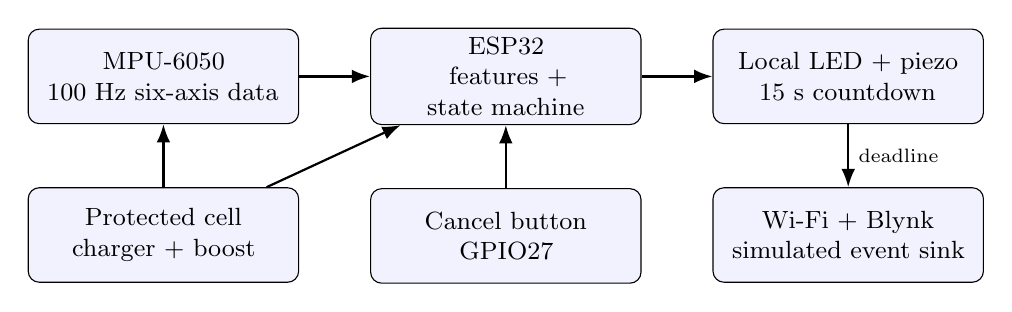
\begin{tikzpicture}[node distance=8mm and 9mm,b/.style={draw,rounded corners,fill=blue!5,align=center,font=\small,minimum height=12mm,text width=32mm},a/.style={-Latex,thick}]
\node[b](imu){MPU-6050\\100 Hz six-axis data};
\node[b,right=of imu](esp){ESP32\\features + state machine};
\node[b,right=of esp](alarm){Local LED + piezo\\15 s countdown};
\node[b,below=of imu](power){Protected cell\\charger + boost};
\node[b,below=of esp](button){Cancel button\\GPIO27};
\node[b,below=of alarm](cloud){Wi-Fi + Blynk\\simulated event sink};
\draw[a](imu)--(esp);\draw[a](esp)--(alarm);\draw[a](button)--(esp);\draw[a](power)--(imu);\draw[a](power)--(esp);\draw[a](alarm)--node[right,font=\scriptsize]{deadline}(cloud);
\end{tikzpicture}
\caption{Architecture of CrashGuard: acquisition, local decision, cancellation by the rider and the remote event. In the harness an instrumented model of the service takes the place of the event sink.}\label{fig:arch}
\end{figure}

\subsection{Circuit diagram and virtual-hardware image}
Figure~\ref{fig:circuit} gives the circuit at connection level (power conditioning, the sensor, the battery measurement and the warning outputs), with labels marking the common nets. The component values are those used in the DC interface calculation below. The drawing also shows how the transistor drives the piezo.

\begin{figure}[H]\centering\resizebox{\linewidth}{!}{%
\begin{circuitikz}[american,scale=.9,transform shape]
\tikzset{mod/.style={draw,rounded corners,align=center,font=\small,fill=blue!4,minimum height=10mm},lab/.style={font=\scriptsize,fill=white,inner sep=1pt}}
% Power chain, common labelled supply nets.
\node[mod,minimum width=28mm] (cell) at (1.5,12.5) {18650 cell\\2600 mAh};
\node[mod,minimum width=35mm] (charge) at (5.5,12.5) {TP4056 + DW01A\\charge / protect};
\node[mod,minimum width=28mm] (boost) at (11,12.5) {MT3608\\5 V boost};
\draw (cell.east)--(charge.west);
\draw (charge.east) to[spst] (boost.west);
\node[lab] at (8.2,13.1) {master switch};
\draw (boost.east)--(14.5,12.5) node[right,lab]{+5V};
\draw (charge.north)--++(0,.55) node[above,lab]{USB 5 V charging};
\draw (cell.south)--++(0,-.4) node[ground]{};
\draw (charge.south)--++(0,-.4) node[ground]{};
\draw (boost.south)--++(0,-.4) node[ground]{};
\node[lab,anchor=west] at (0,11.25) {All GND nets common. Master switch open during charging. VBAT = switched protected cell output.};
% Controller / sensor interface.
\node[mod,minimum width=30mm,minimum height=24mm] (imu) at (1.8,8.8) {MPU-6050\\GY-521\\0x68};
\node[mod,minimum width=32mm,minimum height=36mm] (esp) at (7.0,8.8) {ESP32\\WROOM-32};
\draw ([yshift=8mm]imu.east)--([yshift=8mm]esp.west) node[midway,lab]{VCC -- 3V3};
\draw (imu.east)--(esp.west) node[midway,lab]{SDA -- GPIO21};
\draw ([yshift=-8mm]imu.east)--([yshift=-8mm]esp.west) node[midway,lab]{SCL -- GPIO22};
\draw (imu.south)--++(0,-.4) node[ground]{};
\draw (esp.south)--++(0,-.4) node[ground]{};
\draw (esp.north)--++(0,.4) node[above,lab]{VIN = +5V};
\node[lab] at (1.8,6.9){100 nF across VCC / GND};
% Battery sensing and decoupling.
\draw (10,10.2) node[above,lab]{VBAT} to[R,l=100 k$\Omega$] (10,8.8) coordinate (adc) to[R,l=100 k$\Omega$] (10,7.2) node[ground]{};
\draw (adc)--(12,8.8) coordinate (cap) -- (13.7,8.8) node[right,lab]{GPIO34};
\draw (cap) to[C,l=100 nF] (12,7.2) node[ground]{};
\draw (14.3,10.5) node[above,lab]{+5V} to[C,l=100 $\mu$F] (14.3,9.4) node[ground]{};
% LED branch.
\node[lab,anchor=west] at (0,5.9){Local warning LED};
\draw (0.3,5.2) node[above,lab]{GPIO26} to[R,l=220 $\Omega$] (2.6,5.2) to[leD,l=red LED] (4.8,5.2) -- (5.4,5.2) node[ground]{};
% Button.
\node[lab,anchor=west] at (0,3.7){Cancel button};
\draw (0.3,2.8) node[above,lab]{GPIO27} to[push button,l=CANCEL] (3,2.8) -- (4,2.8) node[ground]{};
\node[lab,anchor=west] at (0,1.8){GPIO27 uses the ESP32 internal pull-up.};
% Piezo branch with independent supply labels.
\node[npn] (q) at (12,3.1) {};
\draw (8.1,3.1) node[above,lab]{GPIO25} to[R,l=1 k$\Omega$] (q.B);
\draw (q.E)--++(0,-.65) node[ground]{};
\draw (q.C) to[buzzer,l=5 V passive piezo] (12,5.5) -- (12,5.9) node[above,lab]{+5V};
\draw (10.8,3.1) to[R,l_=10 k$\Omega$] (10.8,1.4) node[ground]{};
\node[lab,right] at (12.5,3.1){2N2222};
\node[lab,anchor=west] at (0,.5){Supply, GPIO and ground labels identify electrically common nets. MPU-6050 signal pull-ups use 3.3 V.};
\end{circuitikz}%
}
\caption{Connection-level circuit with power, sensing, battery divider, LED, transistor-driven piezo and cancel input. The master switch is open during charging, since the charger module does not share the load.}\label{fig:circuit}\end{figure}

The GY-521 module works at 3.3 V, for power and for logic. GPIO25 drives the piezo through a 2N2222 transistor with a 1 k$\Omega$ base resistor and a 10 k$\Omega$ pull-down. A 100 nF capacitor goes from the battery divider to ground, and the 5 V rail is decoupled by 100 $\mu$F. We computed DC operating points for 39 combinations of cell voltage (3.0 to 4.2 V) and LED forward drop (1.8, 2.0 and 2.2 V). Over these the ADC input ranges from 1.50 to 2.10 V, the divider draws 15 to 21 $\mu$A and the LED current lies between 5.0 and 6.82 mA. The values are calculated, not measured, and they do not depend on the battery experiment of Section~\ref{sec:power}.

Figure~\ref{fig:vh} is a capture of one executed state and not an arbitrary arrangement of parts. It was taken at the moment of confirmation, 3.610 s into the run. Its annotations give the LED level, the tone frequency, the countdown and the converted battery reading at that instant.

\fig{virtual_hardware.png}{1}{Virtual hardware at the confirmation instant, 3.610 s. Board and peripherals show the state recorded by the harness, i.e.\ LED on, 2400 Hz tone and the countdown running.\label{fig:vh}}

\subsection{Dataset generation and preprocessing}
The primary simulation consists of 675 events of ten seconds each at 100 Hz, which makes 675,000 six-axis samples. There are nine classes with 75 events each. Seven of them are negative (normal riding, potholes, speed breakers, hard braking, sharp turning, a parked tip-over and an impact followed by recovery), and the low-side and high-side crashes are positive. This gives 150 positive and 525 negative events. The generator is fixed by the seed 20260828. A second seed, 20260911, produces another 30 events per class, i.e.\ 270 fresh events and 270,000 samples.

Each event is put together from roll, pitch and yaw profiles, the gravity vector in the body frame, pulses for the manoeuvre or the impact, and noise, bias and clipping. In the body frame of the sensor gravity is
\begin{equation}
\label{eq:gravity}
\widehat{\mathbf g}_b=
\begin{bmatrix}
-\sin\theta\\
\sin\phi\cos\theta\\
\cos\phi\cos\theta
\end{bmatrix}\in\mathbb R^{3\times1},\qquad
\mathbf g_b=g_0\widehat{\mathbf g}_b,\qquad
\|\widehat{\mathbf g}_b\|_2=1,
\end{equation}
where $\phi$ and $\theta$ are the roll and pitch angles in radians, and the three entries follow the $x$, $y$ and $z$ axes of the sensor (subscript $b$ for body frame). The hat marks a unit vector. Thus $\widehat{\mathbf g}_b$ has no dimension and its entries read directly in units of $g$. Multiplying by standard gravity, $g_0=9.80665$ m/s$^2$, gives the physical vector $\mathbf g_b$ in m/s$^2$; note that $g_0$ is a constant and is not fitted. For a level sensor ($\phi=\theta=0$) the vector is $[0,0,1]^{\mathsf T}$. Positive roll gives a positive $y$ component, and positive pitch a negative $x$ component. Yaw does not enter, as a rotation about the vertical leaves the direction of gravity unchanged.

Next, linear pulses for the road surface, the rider's inputs and the impacts are added to this gravity vector. For the gyroscope signals the generator does not simply differentiate the Euler angles. Instead it converts the angle rates $\dot{\boldsymbol\Theta}=[\dot\phi,\dot\theta,\dot\psi]^{\mathsf T}$ into body-frame angular velocities $\boldsymbol\omega=[\omega_x,\omega_y,\omega_z]^{\mathsf T}$ by the standard Tait--Bryan $Z$-$Y$-$X$ (yaw--pitch--roll) relation
\begin{equation}\label{eq:rigid_body}
\begin{bmatrix}\omega_x\\\omega_y\\\omega_z\end{bmatrix}=
\mathbf E(\phi,\theta)\begin{bmatrix}\dot\phi\\\dot\theta\\\dot\psi\end{bmatrix}=
\begin{bmatrix}
1 & 0 & -\sin\theta\\
0 & \cos\phi & \sin\phi\cos\theta\\
0 & -\sin\phi & \cos\phi\cos\theta
\end{bmatrix}
\begin{bmatrix}\dot\phi\\\dot\theta\\\dot\psi\end{bmatrix}.
\end{equation}
Here $\psi$ is the yaw angle and $\mathbf E(\phi,\theta)$ is a $3\times3$ matrix depending only on roll and pitch. If the motorcycle rolls and yaws at once, as it does in a high-side crash, the matrix mixes the angle rates over the three gyroscope axes, and this is what a real body-fixed gyroscope would see. At zero roll and pitch the matrix is the identity and the body rates are just the angle rates.

The event time is drawn uniformly between 3.8 and 5.2 s. For acceleration the bias has standard deviation 0.018 $g$ and the sample noise 0.022 $g$; for angular rate the corresponding values are 0.8 and 1.5 $\degree$/s. Samples are clipped to the full-scale ranges of the sensor. The final roll lies between 48 and 105$\degree$ for low-side crashes and between 70 and 135$\degree$ for high-side ones. Note that the low-side range goes below the 55$\degree$ tilt gate of the detector on purpose, so some low-side crashes cannot be detected by design. Before vector addition and clipping the impact pulses are between 3.0 and 11.5 $g$ for high-side crashes and between 0.8 and 5.5 $g$ for low-side crashes.

For the external signal analysis we load seven critical manoeuvres and four falls from the published PTW supplement~\cite{boubezoul2019dataset}. Only the finite numeric rows are kept. The six channels are filtered against aliasing and resampled from 1 kHz to 100 Hz (polyphase resampling with a Kaiser window); acceleration is converted from m/s$^2$ to $g$ by dividing by 9.80665, and angular rate stays in degrees per second. The four fall windows are centred at 40.132, 34.288, 35.876 and 43.486 s and extend $\pm1.5$ s each. The manoeuvres are used whole, as negative examples. Such short windows test single gates only. They are not a test of the full decision with rest and countdown.

\subsection{Data split and evaluation protocol}
Inside each scenario the primary events are split by the order of generation; the first 45 go to development, the next 15 to validation and the last 15 to test. This gives 405, 135 and 135 events (60, 20 and 20\%). No event is divided between subsets, and the file \texttt{results/splits.csv} lists every assignment.

CrashGuard is a fixed set of rules without fitted weights. The split is therefore just a retrospective breakdown of one replay, and the test subset should not be read as a held-out test in the usual sense. The fresh set of 270 events was generated after the detector had been frozen for this study, and no threshold was chosen by looking at it. It is a second random stream from the same family of scenarios. The public PTW recordings are kept for the gate analysis, and the human-fall datasets serve only as context.

\subsection{Features, calibration, and decision equations}
At start-up the firmware averages 200 stationary samples. Calibration is repeated if the norm of the averaged acceleration falls outside 0.85--1.15 $g$, or if the RMS of the gyroscope is above 5 $\degree$/s. Otherwise the averaged acceleration is taken as the reference gravity vector and the three gyroscope means become bias offsets. Let $\mathbf a=[a_x,a_y,a_z]^{\mathsf T}$ be the acceleration vector and $\mathbf r=[r_x,r_y,r_z]^{\mathsf T}$ the reference gravity vector, both in units of $g$, and let $\boldsymbol\omega=[\omega_x,\omega_y,\omega_z]^{\mathsf T}$ be the angular rates in degrees per second. The detector works with three scalar features. The first one is the acceleration magnitude
\begin{equation}\label{eq:accel}
A=\|\mathbf a\|_2=\sqrt{a_x^2+a_y^2+a_z^2},
\end{equation}
where $a_x$, $a_y$ and $a_z$ are the components sampled at the same instant, divided by $g_0$. So $A=1$ stands for one $g$, and the thresholds 2.0 and 0.35 used below mean $2g$ and $0.35g$. The firmware divides the raw signed counts by 2048 counts per $g$ (the scale of the $\pm16g$ range), and a new sample comes every 10 ms.

The second feature is the magnitude of the angular rate,
\begin{equation}\label{eq:rotation}
\Omega=\|\boldsymbol\omega\|_2=\sqrt{\omega_x^2+\omega_y^2+\omega_z^2},
\end{equation}
where $\omega_x$, $\omega_y$ and $\omega_z$ are the bias-corrected rates about the three sensor axes, in degrees per second. Raw values are divided by 16.4 counts per degree per second (the $\pm2000\degree$/s range), and then the calibration means are subtracted. Because of the norm the gate does not care which axis carries the dominant rotation, nor what its sign is. The detector compares $\Omega$ with 90$\degree$/s in the search for a rotation and with 30$\degree$/s in the check for rest; these are thresholds and do not belong to the formula.

The third feature is the tilt, that is the angle between the present acceleration vector and the reference,
\begin{equation}\label{eq:tilt}
\Theta=\frac{180}{\pi}\arccos\!\left[\operatorname{clip}\left(\frac{\mathbf a^{\mathsf T}\mathbf r}{\|\mathbf a\|_2\|\mathbf r\|_2},-1,1\right)\right],
\end{equation}
where $\mathbf a^{\mathsf T}\mathbf r=a_xr_x+a_yr_y+a_zr_z$ is the dot product, $\mathbf r$ is the mean of the 200 accepted calibration samples, and $\operatorname{clip}(u,-1,1)=\min(1,\max(-1,u))$. Division by the two norms gives the cosine of the angle. The clipping guards $\arccos$ against round-off just outside its domain, and the factor $180/\pi$ turns radians into degrees, so that $\Theta\in[0,180]$. When the product of the norms is below $10^{-6}$ the implementation returns zero tilt. As $\Theta$ is computed from the instantaneous acceleration, it gives the lean of the vehicle properly only while the motion is small. This is the case during the rest after a fall, and that is where we use it.

The decision then goes as follows. Riding activity is present if $|A-1|\geq0.08$ or $\Omega\geq4\degree$/s. Activity evidence builds up to 1000 ms and decays at half that rate when there is no activity; as long as the evidence is full, a 5000 ms deadline for active riding is refreshed. Once riding is qualified, a candidate begins when $A\geq2.0$ or $A\leq0.35$. Within 750 ms of the candidate there must be a rotation with $\Omega\geq90\degree$/s. After this the detector waits for the rest condition
\begin{equation}
 \label{eq:rest} R=(\Theta\geq55\degree)\land(0.70\leq A\leq1.30)\land(\Omega\leq30\degree/\mathrm{s}),
\end{equation}
where $\land$ denotes logical AND. Thus $R$ holds only when the motorcycle is strongly tilted, the acceleration is near $1g$ (within $\pm0.30g$) and the vehicle hardly rotates. All comparisons include their limits. The predicate is instantaneous; the time requirements are imposed by the state machine and not by Equation~\eqref{eq:rest}.

A crash is confirmed once $R$ has held for 2000 ms, and verification is given up 6000 ms after the candidate. Confirmation starts the alarm and the 15,000 ms cancellation window. The state machine needs only constant memory and does constant amount of work per sample.

\subsection{Algorithm and flowchart}
Table~\ref{tab:algo} lists the firmware procedure in the order in which it runs, from sensor initialisation to the single event submission, and shows where a failure of the sensor or the network changes the normal path.

\begin{table}[H]\centering\small\caption{Algorithm 1: firmware procedure from sensor initialisation to the one-shot incident submission. Each row is one step of the implemented control path, together with its timing or failure branch. Samples are taken every 10 ms (100 Hz) and calibration uses 200 samples. If a sensor read fails the detector update is skipped. The deadline step records the outcome at the service, which does not imply that a notification reached anyone.}\label{tab:algo}
\begin{tabularx}{\linewidth}{|c|X|}\hline
\textbf{Step} & \textbf{Operation}\\\hline
1 & Configure the GPIO pins and the MPU-6050; if the sensor does not answer, stop safely.\\\hline
2 & Collect 200 samples. If the device moved or the data are invalid, repeat until a valid reference is found.\\\hline
3 & Start Wi-Fi association in the background and set up the 10 ms sampling schedule.\\\hline
4 & Look for a press of the cancel button. It cancels a running countdown, or acknowledges an alert and silences the outputs.\\\hline
5 & At each sampling deadline read the 14-byte sensor burst. On failure log a warning and skip the detector update.\\\hline
6 & Compute $A$, $\Omega$ and $\Theta$, then update the activity evidence and the candidate, rotation and rest states.\\\hline
7 & On confirmation set the LED high, start the 2400 Hz tone and note the start of the countdown.\\\hline
8 & After 15 s perform one event operation and record whether it was submitted, disabled, skipped for lack of Wi-Fi or skipped for lack of cloud.\\\hline
9 & Keep the local warning on until the rider acknowledges it, and go on sampling.\\\hline
\end{tabularx}\end{table}

The flowchart of Figure~\ref{fig:flow} gives the same procedure as a chain of decisions with two return paths. A rejected candidate goes back to sampling, and a cancellation by the rider stops the warning before the event falls due.

\begin{figure}[H]\centering
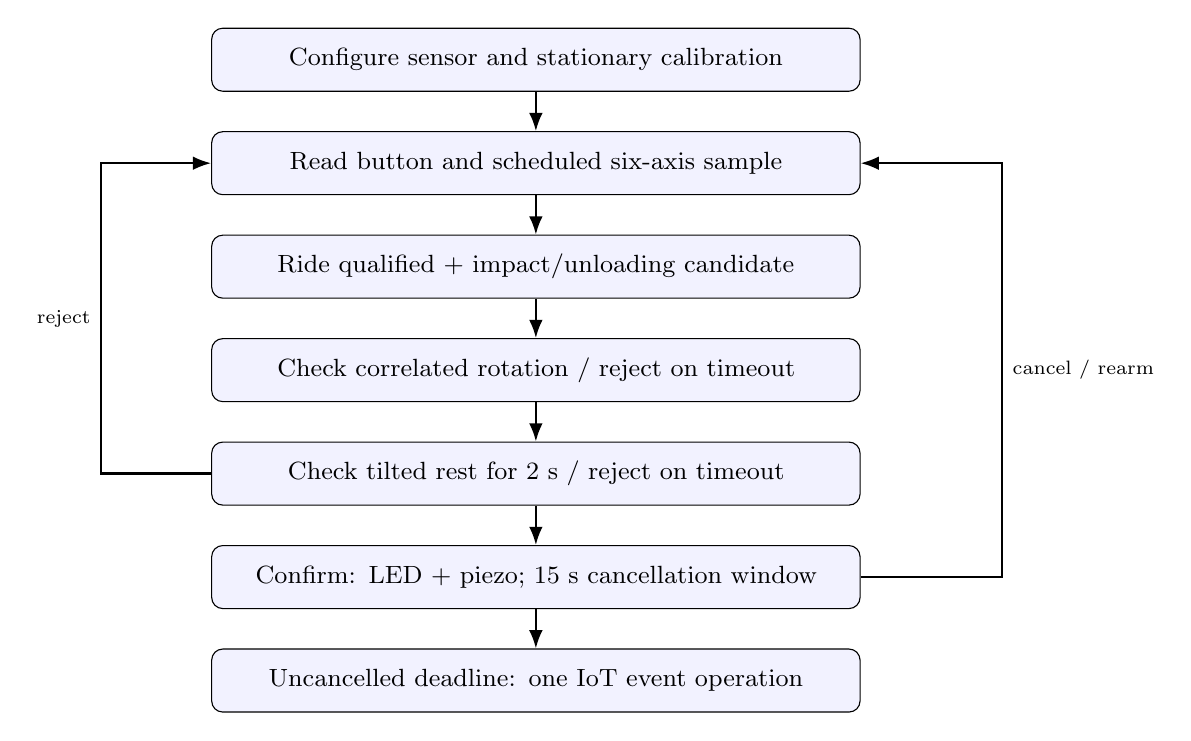
\begin{tikzpicture}[node distance=5mm,b/.style={draw,rounded corners,fill=blue!5,align=center,text width=80mm,minimum height=8mm,font=\small},a/.style={-Latex,thick}]
\node[b](start){Configure sensor and stationary calibration};
\node[b,below=of start](sample){Read button and scheduled six-axis sample};
\node[b,below=of sample](ride){Ride qualified + impact/unloading candidate};
\node[b,below=of ride](rot){Check correlated rotation / reject on timeout};
\node[b,below=of rot](rest){Check tilted rest for 2 s / reject on timeout};
\node[b,below=of rest](count){Confirm: LED + piezo; 15 s cancellation window};
\node[b,below=of count](event){Uncancelled deadline: one IoT event operation};
\foreach \a/\b in {start/sample,sample/ride,ride/rot,rot/rest,rest/count,count/event}\draw[a](\a)--(\b);
\draw[a](count.east)--++(18mm,0)|-node[pos=.25,right,font=\scriptsize]{cancel / rearm}(sample.east);
\draw[a](rest.west)--++(-14mm,0)|-node[pos=.25,left,font=\scriptsize]{reject}(sample.west);
\end{tikzpicture}\caption{Flowchart of a successful detection, with the return paths for rejection and for cancellation. A failed sensor read also goes back to the sampling loop.}\label{fig:flow}
\end{figure}

\subsection{Baselines and metrics}\label{sec:baselines}
We compare CrashGuard with three other rules. The \emph{acceleration-only} rule fires as soon as $A\geq2.0$. The \emph{strict ordered} rule asks for $A\geq4.0$, then $\Omega\geq200\degree$/s within 500 ms, and then a tilt of at least 60$\degree$ with $0.70\leq A\leq1.30$ held for three seconds, all of it within eight seconds of the impact. The third rule follows the staged structure of the motorcycle fall detector of Boubezoul et al.~\cite{boubezoul2013algorithm}, and we call it by their name. It has three stages. A fall starts when the roll rate $|\omega_x|$ reaches 60$\degree$/s, or when $A\geq2.5$ or $A\leq0.40$. The lean must then reach $\Theta\geq55\degree$ within 2 s, or else the rule resets. Lastly the rest condition $\Theta\geq55\degree$, $0.70\leq A\leq1.30$, $\Omega\leq30\degree$/s has to hold without a break for 1.5 s, and the attempt is given up 6 s after the start. We should be clear that these thresholds are our own choices, written to follow the structure of the published method. We do not claim that they are the exact values of the original paper, so the rule approximates their detector and is not a copy of it. Unlike CrashGuard it has no ride qualification.

Let $TP$, $TN$, $FP$ and $FN$ denote the numbers of true positives, true negatives, false positives and false negatives. They all count whole events, and in every experiment below the denominators of the metrics are positive. The first metric is accuracy,
\begin{equation}\label{eq:accuracy} \mathrm{Accuracy}=\frac{TP+TN}{TP+TN+FP+FN},\end{equation}
the fraction of all events classified correctly. Its denominator is the size $N$ of the evaluation set ($N=675$ for the primary set, $N=270$ for the fresh set). Negative events far outnumber positive ones, so accuracy can be high even when many crashes are missed. For this reason we never report it alone.

Sensitivity (also called recall, or the true-positive rate) is the fraction of crashes which are detected,
\begin{equation}\label{eq:sensitivity} \mathrm{Sensitivity}=\frac{TP}{TP+FN}.\end{equation}
The denominator is the number of labelled crashes, 150 in the primary set and 60 in the fresh one. This metric shows missed crashes directly, and we also give it separately for low-side and high-side crashes. For instance the fresh CrashGuard result is $43/(43+17)=0.717$, or 71.7\%.

Specificity is the fraction of non-crash events correctly rejected,
\begin{equation}\label{eq:specificity} \mathrm{Specificity}=\frac{TN}{TN+FP},\end{equation}
with 525 negatives in the primary set and 210 in the fresh set. It describes nuisance alarms, but only within the negative events we chose to generate, and so it must be read together with how many such events there are and how varied they are. For the fresh CrashGuard result $TN=210$ and $FP=0$, and the observed value is 1. This is a finite sample. Rather than claim perfect rejection we give a Wilson interval for it below.

Precision is the fraction of detections which are real crashes,
\begin{equation}\label{eq:precision} \mathrm{Precision}=\frac{TP}{TP+FP}.\end{equation}
Its denominator counts all events predicted positive, whatever their true class, so precision depends on how common crashes are in the test set. If a rule predicted no positive event at all the ratio would be undefined, and our code would return zero; this does not happen in any result reported here. For CrashGuard on the fresh set the precision is $43/(43+0)=1$.

The F1-score combines precision and sensitivity,
\begin{equation}\label{eq:f1} F_1=\frac{2TP}{2TP+FP+FN},\end{equation}
that is, the harmonic mean of the two expressed through counts (the subscript 1 means that both are weighted equally). F1 is penalised by either kind of error. We report it as a decimal between 0 and 1, while accuracy, sensitivity and specificity are given in percent. For the fresh CrashGuard counts $F_1=86/103=0.835$.

The false-positive rate is
\begin{equation}\label{eq:fpr} \mathrm{FPR}=\frac{FP}{TN+FP},\end{equation}
the fraction of non-crash events which raise an alarm, i.e.\ one minus the specificity. For the acceleration-only rule on the fresh set $FP=108$ and $TN=102$, so $\mathrm{FPR}=108/210=51.4\%$; for CrashGuard the numerator is zero. Note that this is a rate per event. A rate of false alarms per hour of riding would need riding time in the denominator, and our data do not give it.

The delay of a detection is the confirmation time minus the time at which the successful candidate began, and it is computed for detected crashes only. We briefly note that the acceleration-only rule has, by definition, no confirmation hold and hence zero delay. For a proportion $\hat p=x/n$ with $x$ successes in $n$ events we give 95\% Wilson intervals~\cite{wilson1927interval},
\begin{equation}\label{eq:wilson}
\begin{aligned}
p_{\mathrm L}&=\frac{\hat p+z^2/(2n)-z\sqrt{\hat p(1-\hat p)/n+z^2/(4n^2)}}{1+z^2/n},\\[2mm]
p_{\mathrm U}&=\frac{\hat p+z^2/(2n)+z\sqrt{\hat p(1-\hat p)/n+z^2/(4n^2)}}{1+z^2/n},
\end{aligned}
\end{equation}
where $p_{\mathrm L}$ and $p_{\mathrm U}$ are the lower and upper limits, and $z=1.959964$ is the 97.5th percentile of the standard normal distribution. For sensitivity $x=TP$ and $n=TP+FN$; for specificity $x=TN$ and $n=TN+FP$. The constants 2 and 4 come from the Wilson score construction. Unlike the simple normal interval, the Wilson interval remains informative when every observed event is a success, which is the case for our specificity. The intervals describe the uncertainty due to the finite number of events. Whether the generator resembles real riding is a separate matter, and on this they say nothing.

Finally, to test whether two rules differ on the same events we use McNemar's test with Edwards' continuity correction~\cite{mcnemar1947},
\begin{equation}\label{eq:mcnemar}
\chi^2 = \frac{(|b - c| - 1)^2}{b + c},
\end{equation}
where $b$ is the number of events which CrashGuard gets right and the other rule gets wrong, and $c$ is the number for which it is the other way round. Events on which the two rules agree play no part in the statistic. Under the null hypothesis that the two rules have equal error rates, $\chi^2$ follows a chi-squared distribution with one degree of freedom. With few discordant events ($b+c<25$) we use the exact two-sided binomial $p$-value instead, $p = 2 \sum_{k=0}^{\min(b,c)} \binom{b+c}{k} 0.5^{b+c}$.

\section{Experimental Results and Discussion}
\subsection{Experimental conditions}
The C++17 programs are compiled with optimisation and strict warnings. Python with NumPy, SciPy and Matplotlib is used to generate the data, replay the detector, compute the metrics and draw the plots. Each event is processed by a freshly reset detector. The firmware harness has a virtual clock, a 14-byte register buffer, instrumented GPIO and tone outputs and a local Blynk-compatible sink. It runs the unchanged firmware and, on request, returns a failed probe, a truncated read, a lost link or a cloud timeout. No network credentials are needed.

We re-ran the pipeline on the 675 primary events and got the same confusion counts as before. Then we added the 270 fresh events, so that in total 945 events and 945,000 samples were processed. Besides these we ran 14 firmware scenarios, 39 DC operating points and nine battery-discharge cases. The experiments test different layers of the system and their counts are reported separately.

\subsection{Original and fresh performance comparison}
Table~\ref{tab:orig} compares the four rules on the 675 primary events, and from its confusion counts one can see where each score comes from. CrashGuard rejects far more non-crash events than the acceleration-only and the Boubezoul rules. The strict ordered rule also rejects every negative event, but it loses many more crashes.

\begin{table}[H]\centering\small\caption{Event-level comparison of the four rules on the same 675 primary events (seed 20260828; 150 crashes and 525 non-crash events). TP, TN, FP and FN count events. Acc., Sens. and Spec. stand for accuracy, sensitivity and specificity in percent, and F1 is in $[0,1]$. Each row sees identical input, so the differences are due to the rules alone.}\label{tab:orig}
\resizebox{\linewidth}{!}{\begin{tabular}{|l|r|r|r|r|r|r|r|r|}\hline
\textbf{Detector} & \textbf{TP} & \textbf{TN} & \textbf{FP} & \textbf{FN} & \textbf{Acc. (\%)} & \textbf{Sens. (\%)} & \textbf{Spec. (\%)} & \textbf{F1}\\\hline
Acceleration-only & 134 & 236 & 289 & 16 & 54.8 & 89.3 & 45.0 & 0.468\\\hline
Strict ordered & 39 & 525 & 0 & 111 & 83.6 & 26.0 & 100.0 & 0.413\\\hline
Boubezoul et al. (2013) & 135 & 436 & 89 & 15 & 84.6 & 90.0 & 83.0 & 0.722\\\hline
CrashGuard (Ours) & 114 & 525 & 0 & 36 & 94.7 & 76.0 & 100.0 & 0.864\\\hline
\end{tabular}}\end{table}

Table~\ref{tab:fresh} repeats the comparison on the 270 fresh events, with the rules unchanged. What we want to know is whether the pattern of the primary set survives on a new random stream. No threshold was chosen by looking at these results.

\begin{table}[H]\centering\small\caption{The unchanged rules on 270 fresh events (seed 20260911; 60 crashes and 210 non-crash events). Columns are as in Table~\ref{tab:orig}. This is a test of repeatability within the same generator, not a validation on other vehicles or road sessions.}\label{tab:fresh}
\resizebox{\linewidth}{!}{\begin{tabular}{|l|r|r|r|r|r|r|r|r|}\hline
\textbf{Detector} & \textbf{TP} & \textbf{TN} & \textbf{FP} & \textbf{FN} & \textbf{Acc. (\%)} & \textbf{Sens. (\%)} & \textbf{Spec. (\%)} & \textbf{F1}\\\hline
Acceleration-only & 52 & 102 & 108 & 8 & 57.0 & 86.7 & 48.6 & 0.473\\\hline
Strict ordered-threshold & 12 & 210 & 0 & 48 & 82.2 & 20.0 & 100.0 & 0.333\\\hline
Boubezoul et al. (2013) & 52 & 176 & 34 & 8 & 84.4 & 86.7 & 83.8 & 0.712\\\hline
CrashGuard (Ours) & 43 & 210 & 0 & 17 & 93.7 & 71.7 & 100.0 & 0.835\\\hline
\end{tabular}}\end{table}

On the primary set CrashGuard removes all 289 false alarms of the acceleration-only rule, and misses 20 more crashes than that rule does. Compared with the Boubezoul rule it removes 89 false alarms (specificity 100.0\% against 83.0\%) and misses 21 more crashes (sensitivity 76.0\% against 90.0\%). On the fresh set the pattern is the same. CrashGuard has none of the 34 false alarms of the Boubezoul rule, which lifts specificity from 83.8\% to 100.0\% and accuracy from 84.4\% to 93.7\% (F1 0.835 against 0.712), but it misses 9 more low-side crashes (71.7\% against 86.7\%). So neither rule dominates the other. CrashGuard pays for its silence on non-crash events with missed slow crashes. Whether this is the right trade depends on how riders react to repeated false alarms, and our data cannot answer that.

McNemar's test confirms that the errors of CrashGuard and of the Boubezoul rule are significantly different, with $\chi^2=40.81$ ($p=1.68\times10^{-10}$) on the primary set and $\chi^2=13.40$ ($p=0.00025$) on the fresh set. This needs to be read with some care, however. On the fresh set the discordant events are 34 non-crash events which only the Boubezoul rule gets wrong, and 9 crashes which only CrashGuard misses. The significance thus mostly reflects the false alarms of the Boubezoul rule, and it is no evidence that CrashGuard detects crashes better. Against the strict ordered rule CrashGuard detects significantly more crashes with no extra false alarm ($\chi^2=73.01$, $p<10^{-15}$ on the primary set; $\chi^2=29.03$, $p=7.1\times10^{-8}$ on the fresh set). Against the acceleration-only rule the difference is larger again ($\chi^2=232.44$, $p<10^{-15}$ on the primary set; $\chi^2=82.09$, $p<10^{-15}$ on the fresh set).

For the fresh set the 95\% Wilson interval of sensitivity is 59.2--81.5\%, and the observed specificity of 100.0\% has the interval 98.2--100.0\%. On the primary set the intervals are 68.6--82.1\% for sensitivity and 99.3--100.0\% for specificity. That no false alarm was seen in a finite set of negatives does not mean that none would occur under any riding condition.

The CrashGuard counts for each subset of the data are in Table~\ref{tab:split}. The table keeps the retrospective development, validation and test breakdown of the primary set apart from the fresh-seed experiment, as the two play different roles.

\begin{table}[H]\centering\small\caption{CrashGuard confusion counts and F1 for each whole-event subset. Within each of the nine scenarios the primary simulation is split into 45 development, 15 validation and 15 test events (405/135/135 in total). The fresh-seed set adds 30 events per scenario. TP, TN, FP and FN sum to the number of events. The rules are fixed, so no weights are fitted in any subset.}\label{tab:split}
\begin{tabular}{|l|r|r|r|r|r|r|}\hline
\textbf{Partition} & \textbf{Events} & \textbf{TP} & \textbf{TN} & \textbf{FP} & \textbf{FN} & \textbf{F1}\\\hline
Development & 405 & 67 & 315 & 0 & 23 & 0.854\\\hline
Validation & 135 & 23 & 105 & 0 & 7 & 0.868\\\hline
Retrospective test & 135 & 24 & 105 & 0 & 6 & 0.889\\\hline
Fresh-seed test & 270 & 43 & 210 & 0 & 17 & 0.835\\\hline
\end{tabular}\end{table}

The F1 values of the three primary subsets are between 0.854 and 0.889, and the fresh value of 0.835 is slightly lower. With 30 positives or fewer in a subset, differences of this size are to be expected.

\subsection{Scenario analysis and graphs}
All seven negative classes are rejected completely in both sets, and no high-side crash is missed (75 of 75 are detected in the primary set and 30 of 30 in the fresh set). For low-side crashes the counts are 39 of 75 and 13 of 30. Hence each of the 36 primary misses and of the 17 fresh misses is a low-side crash. The low-side profiles have weaker impacts, slower motion and a smaller final lean than the high-side profiles, and the fixed gates accept only part of that distribution.

Figure~\ref{fig:scen} gives the fraction of correct decisions per class in both sets. What it shows is simple. Overall accuracy hides one class which fails often, the other eight being handled without a single error in these finite sets.

\fig{scenarios.pdf}{1}{Fraction of correct event decisions per scenario, for the primary replay (left; 75 events per class) and for the fresh-seed set (right; 30 events per class). Crash classes are in orange and non-crash classes in blue.\label{fig:scen}}

Figure~\ref{fig:prof} plots the three features against time for one generated pothole, one parked tip-over and one low-side crash. The pothole gives a sharp acceleration peak above 3$g$, but its rotation stays close to the 90$\degree$/s line and the tilt does not rise at all. The parked tip-over and the crash both rotate fast and end up strongly tilted. What separates them is the ride qualification, as the tip-over happens with no riding before it. This is why the same peak value need not lead to the same decision.

\fig{simulated_profiles.pdf}{.95}{Acceleration magnitude $\|\mathbf a\|$ (top), angular-rate magnitude $\|\boldsymbol\omega\|$ (middle) and tilt (bottom) for a generated pothole, a parked tip-over and a low-side crash. The dashed lines mark the 2$g$, 90$\degree$/s and 55$\degree$ thresholds.\label{fig:prof}}

In Figure~\ref{fig:conf} the fresh confusion matrix is placed next to the distribution of confirmation delays. Note that the two panels have different denominators; the matrix counts all 270 events, the histogram only the 43 detected crashes. Most delays are between 2.2 and 2.4 s, just above the 2 s rest hold.

\fig{confusion_delay.pdf}{1}{Confusion matrix of the fresh set (left) and the candidate-to-confirmation delays of the 43 detected crashes (right). Missed crashes appear in the matrix only.\label{fig:conf}}

\subsection{External public-data gate analysis}
Table~\ref{tab:ext} summarises the four public fall windows after unit conversion and resampling. From the peak and minimum acceleration we see whether the unloading gate opens, and from the peak angular rate whether the rotation gate opens. The last column records only that both gates are crossed at some point in the window. It does not say that the full decision would be made.

\begin{table}[H]\centering\small\caption{Extremes of the inertial signals in four public PTW fall windows, after anti-aliased resampling from 1 kHz to 100 Hz. Each row covers 3 s centred on the event. Peak and minimum $A$ are in $g$, and peak $\Omega$ in degrees per second. ``Both gates'' means that the acceleration condition ($A\geq2.0$ or $A\leq0.35$) and the rotation condition ($\Omega\geq90\degree$/s) are each met somewhere in the window. It says nothing about their timing, nor about the rest condition.}\label{tab:ext}
\begin{tabularx}{\linewidth}{|X|r|r|r|c|}\hline
\textbf{Fall recording} & \textbf{Peak $A$ ($g$)} & \textbf{Min. $A$ ($g$)} & \textbf{Peak $\Omega$ ($\degree$/s)} & \textbf{Both gates}\\\hline
Slippery straight road & 1.169 & 0.013 & 179.4 & Yes\\\hline
Leaning motorcycle & 1.878 & 0.041 & 144.1 & Yes\\\hline
Roundabout & 1.690 & 0.011 & 150.5 & Yes\\\hline
Curve & 1.436 & 0.130 & 151.6 & Yes\\\hline
\end{tabularx}\end{table}

All four falls open both CrashGuard gates. In every case it is the unloading branch ($A\leq0.35$) which opens, as no peak reaches $2g$. None of the falls reaches the 4$g$ and 200$\degree$/s gates of the strict rule, and this explains part of its poor recall. On the other hand, three of the seven manoeuvres (accelerating in a curve, accelerating on a straight line and hard braking) also open both CrashGuard gates somewhere in their recordings. The gates by themselves do not, therefore, separate falls from manoeuvres. That is left to the requirements on timing, riding and rest, which we cannot check on these recordings since the fall windows are short. The full features of all eleven recordings are in \texttt{external\_ptw\_features.csv}.

\subsection{Timing, cancellation, and IoT communication}
From candidate to confirmation the median delay is 2315 ms on the primary set and 2330 ms on the fresh set. The strict ordered rule needs 3120 and 3130 ms, the Boubezoul rule 2280 and 2325 ms. Most of the delay is thus due to the rest hold itself. Adding the intentional 15 s cancellation window, the time from the candidate to the event deadline at the fresh median is 17.33 s, before any delay in connecting to the service.

In the harness riding is qualified first. A rotation is then injected at 1500 ms and an impact at 1600 ms. The tilted rest starts at 1610 ms, confirmation comes at 3610 ms and the event falls due at 18,610 ms. The test checks that the state is still \texttt{COUNTDOWN} at 18,600 ms and has become \texttt{ALERT\_DUE} ten milliseconds later. After confirmation GPIO26 is high and the tone is at 2400 Hz. The simulated service receives exactly one \texttt{crash\_confirmed} event, with a description 143 bytes long.

In another test the cancel button on GPIO27 is pressed at 4010 ms. The outputs switch off and the detector stays idle until the run ends at 20,000 ms. Four outcomes are distinguished on the event path: submission to the service, a disabled configuration, a Wi-Fi failure and a cloud failure. The event description gives the acceleration, angular rate and tilt at confirmation, and says that no location fix is available (the device has no GNSS receiver). Event identity and payload follow the Blynk firmware event interface~\cite{blynkevents}.

Taken together, the virtual-hardware image and the state traces work as a replay dashboard, in which the sensor values, the countdown, the alarm outputs and the event outcome all come from one run. A deployed application could show the same fields through a Blynk device template. Continuous telemetry on virtual pins would be an extension. In the sketch evaluated here the only remote operation is the event submission.

\subsection{Threshold sensitivity and calibration analysis}
To see how much the results depend on the chosen thresholds we varied one parameter at a time, with the others at their configured values, and replayed the 675 primary events for each setting. Parameters and ranges were as follows.
\begin{enumerate}
\item The rest tilt threshold $\Theta_{\mathrm{tilt}}$; 13 values from 40$\degree$ to 70$\degree$ in steps of 2.5$\degree$.
\item The rotation gate $\Omega_{\mathrm{rot}}$; 10 values from 60 to 150$\degree$/s in steps of 10$\degree$/s.
\item The rest hold $T_{\mathrm{hold}}$; 6 values from 1.0 to 3.5 s in steps of 0.5 s.
\end{enumerate}
In all this makes 29 settings. The sweep reuses the events on which the configuration was developed, so it describes how the rules behave and is not an independent test. Figure~\ref{fig:sensitivity} shows the results.

\begin{figure}[H]\centering
\safeincludegraphics[width=\linewidth]{threshold_sensitivity.pdf}
\caption{One-at-a-time threshold sweeps on the 675 primary events: (a) rest tilt threshold, (b) rotation gate, (c) rest hold. Each panel gives overall sensitivity, low-side recall and specificity, and the dotted line marks the configured value (55$\degree$, 90$\degree$/s, 2.0 s).}\label{fig:sensitivity}
\end{figure}

\textbf{Tilt.} For every tilt threshold down to 50$\degree$ specificity stays at 100\%. From 47.5$\degree$ down, two non-crash events are accepted (99.6\%). Inside the range free of false alarms the tilt threshold matters surprisingly little; sensitivity is 76.7\% at 50--52.5$\degree$ and 76.0\% from 55$\degree$ to 62.5$\degree$, a difference of one event. Going down to 45$\degree$ wins back four more low-side crashes (low-side recall 57.3\%, overall 78.7\%), at the price of the two false alarms. Above 62.5$\degree$ sensitivity drops, and at 67.5$\degree$ and 70$\degree$ even high-side crashes start to be lost (98.7\% and 96.0\%); at 70$\degree$ the overall sensitivity is 70.7\%. Our conclusion is that the tilt gate is not the main cause of the low-side misses.

\textbf{Rotation.} Over the whole range from 60 to 150$\degree$/s specificity stays at 100\%, while low-side recall depends strongly on the gate. It is 62.7\% at 60 and 70$\degree$/s, 52.0\% at the configured 90$\degree$/s and just 10.7\% at 150$\degree$/s. On these data, then, a rotation gate of 70$\degree$/s would detect eight more low-side crashes (overall sensitivity 81.3\% in place of 76.0\%) without one false alarm. This is perhaps the most useful outcome of the sweep, as it shows that the configured point is not the best of those free of false alarms. We have kept the configuration as it is, however. The observation comes from the development data, and the rejection of negatives may rest largely on the other conditions; before a lower rotation gate is adopted it has to be checked on held-out events.

\textbf{Rest hold.} Here it is the other way round. Sensitivity hardly changes (76.7\% at 1.0 and 1.5 s, 76.0\% from 2.0 s on), but specificity falls to 97.7\% (12 false alarms) at 1.5 s and to 96.0\% (21 false alarms) at 1.0 s. The sweep does not record which classes these false alarms come from. A likely source is the impact-with-recovery class, whose generated lean lasts 0.7 to 2.1 s, but we have not verified this. Longer holds give no gain in specificity, and since the hold is part of the confirmation delay, each extra half second of hold adds about half a second of delay by construction. Of the holds tried, 2 s is thus the shortest one which removes all false alarms.

\subsection{Firmware implementation verification and code defect discovery}
Table~\ref{tab:tests} pairs each injected condition with the intended response and with the trace actually observed. Most cases check that the firmware behaves as specified. Three of them (T9, T11 and T13) isolate defects in this particular code. We stress that these are defects of our prototype implementation and not properties of IoT hardware in general; the harness found them before any board had been flashed.

\small
\begin{longtable}{|>{\raggedright\arraybackslash}p{.05\linewidth}|>{\raggedright\arraybackslash}p{.21\linewidth}|>{\raggedright\arraybackslash}p{.28\linewidth}|>{\raggedright\arraybackslash}p{.35\linewidth}|}
\caption{Fourteen experiments with the exact firmware and deterministic models of the sensor, GPIO, clock and service. ID names the case, Stimulus is the injected input or failure, Expected the required behaviour, and Actual the observed trace with its interpretation. Times are in virtual-clock milliseconds unless written in seconds. Alarm 1/0 means that the local warning is commanded on/off. For T9, T11 and T13 a passing assertion reproduces a known weakness, and does not certify tolerance to faults.}\label{tab:tests}\\
\hline
\textbf{ID} & \textbf{Stimulus} & \textbf{Expected behaviour / criterion} & \textbf{Actual result and interpretation}\\\hline\endfirsthead
\hline
\textbf{ID} & \textbf{Stimulus} & \textbf{Expected behaviour / criterion} & \textbf{Actual result and interpretation}\\\hline\endhead
T1 & Sensor absent at boot & Probe failure; safe stop; alarm off & Fatal marker and safe-stop loop observed; alarm 0. Conforms.\\\hline
T2 & Ten-byte sensor burst & Reject incomplete 14-byte read & Warning emitted; state remains IDLE. Conforms.\\\hline
T3 & I\textsuperscript{2}C error status & Skip invalid sample & Warning emitted; state remains IDLE. Conforms.\\\hline
T4 & 100$\degree$/s during calibration & Reject motion above 5$\degree$/s RMS & Calibration rejected. Conforms.\\\hline
T5 & Stationary gravity input & Accept 200 valid samples & Calibration accepted after 200 samples. Conforms.\\\hline
T6 & ADC returns 1850 mV & Reconstruct cell voltage with factor two & 3.700 V returned. Conforms.\\\hline
T7 & Cancel at 4010 ms & Silence outputs and suppress deadline & Alarm 0; IDLE through 20 s. Conforms.\\\hline
T8 & Uncancelled crash & 15,000 ms from confirmation to one event & 3610 ms confirmation; 18,610 ms deadline; one event. Conforms.\\\hline
T9 & Missing reads during rest & Desired: require continuous valid rest evidence & Confirmation at 3610 ms despite a sample gap. Continuity defect exposed.\\\hline
T10 & Wi-Fi unavailable at deadline & Explicit skip; local alarm kept & Zero sink events; Wi-Fi skip marker; alarm 1. Conforms.\\\hline
T11 & Cloud connection fails & Explicit failure; characterise blocking & Zero sink events; 5000 ms blocking; alarm 1. Blocking risk exposed.\\\hline
T12 & Connected simulated sink & Correct event code and bounded payload & One event; code \texttt{crash\_confirmed}; 143 bytes. Conforms.\\\hline
T13 & Wi-Fi recovers after deadline & Desired: eventual incident delivery & Zero events after recovery. Missing retry exposed.\\\hline
T14 & Build without credentials & Disabled marker; local alarm kept & Not-configured marker; alarm 1. Conforms.\\\hline
\end{longtable}
\normalsize

All fourteen assertions pass. For T9, T11 and T13, passing means that the known defect is reproduced. We go through the three defects in turn.

\textbf{T9: rest-timer continuity.} The rest timer measures the time elapsed between timestamps, without checking that samples actually arrived in between. If the I\textsuperscript{2}C reads fail during the rest, time still counts. In the test a valid rest sample at 1610 ms is followed by bus failures at 2000 and 3000 ms and then by a valid sample at 3610 ms. The crash is confirmed, although the sensor was silent for 2000 ms. The fix is to restart the rest timer whenever the gap between valid samples is longer than, say, 50 ms.

\textbf{T11: blocking connection.} The cloud connection call is synchronous, with a 5000 ms timeout. If the service cannot be reached the call holds the main loop for those 5 s, and sampling deadlines are missed. Production firmware needs a non-blocking network state machine.

\textbf{T13: no retry.} An incident which falls due while Wi-Fi is down is skipped, and the state moves on to \texttt{ALERT\_COMPLETED}. Nothing is sent when Wi-Fi comes back. The event must be stored and retried.

The GPIO and tone assertions are about the commanded outputs only. The present firmware gets no feedback from its actuators, so it cannot detect a disconnected piezo or a dead LED. Checking that the outputs physically work would need extra sensing, which we leave for future work.

\subsection{Expected performance versus actual performance}
Table~\ref{tab:goals} puts each design objective next to the experiment which tests it, and says what follows. Classification, timing, recovery and endurance appear side by side, the objectives which were not met included.

\begin{table}[H]\centering\small\caption{Objectives, observations and interpretation. The classification rows give correct decisions or false alarms over the relevant number of events in the primary and fresh sets. The timing rows use the virtual clock of the firmware, and the recovery rows say whether continuous rest evidence and eventual delivery are achieved. The endurance row is for the 120 mA, 5 V, 90\% efficiency case. Meeting one row does not mean that the others are met.}\label{tab:goals}
\begin{tabularx}{\linewidth}{|>{\raggedright\arraybackslash}p{.26\linewidth}|>{\raggedright\arraybackslash}p{.36\linewidth}|X|}\hline
\textbf{Objective} & \textbf{Actual experiment} & \textbf{Interpretation}\\\hline
Reject road disturbances & 0/525 primary and 0/210 fresh false alarms & Achieved in both scenario sets.\\\hline
Detect crash-like events & 114/150 primary; 43/60 fresh & Low-side sensitivity is the main weakness.\\\hline
Allow cancellation & Alarm silenced at 4010 ms; IDLE through 20 s & Cancellation conforms.\\\hline
Enforce 15 s alert interval & 18,610 $-$ 3610 = 15,000 ms & Exact deadline on the virtual clock.\\\hline
Keep valid rest evidence & Sensor gap spans the rest timer & Timer must restart after a gap.\\\hline
Recover event delivery & Zero events after the link returns & Persistent retry needed.\\\hline
Run for 12 h in the nominal case & 12.64 h at 120 mA and 90\% efficiency & Met in the nominal case; heavier loads fall short.\\\hline
\end{tabularx}\end{table}

\subsection{Power simulation}\label{sec:power}
The battery is modelled as a reservoir of usable charge which is drawn down step by step. The operating time comes out of the model; it is not put into it. The initial charge is
\begin{equation}\label{eq:charge_initial}
q_0=C_{\mathrm{nom}}f_{\mathrm{use}}=(2.6\,\mathrm{Ah})(0.90)=2.34\,\mathrm{Ah},
\end{equation}
where $C_{\mathrm{nom}}=2.6$ Ah is the nominal capacity of the cell, $f_{\mathrm{use}}=0.90$ is the fraction of it we treat as usable, and the subscript 0 marks the start of discharge. Both inputs are fixed parameters of the simulation.

While the cell discharges, its voltage falls linearly with the remaining charge,
\begin{equation}\label{eq:cell_voltage}
V(q)=V_{\min}+(V_{\max}-V_{\min})\frac{q}{q_0}
     =3.0\,\mathrm V+(1.2\,\mathrm V)\frac{q}{q_0},
\end{equation}
where $q$ is the remaining usable charge in Ah, with $0\leq q\leq q_0$, so that $q/q_0$ is the state of charge. The voltage is $V_{\min}=3.0$ V for an empty cell and $V_{\max}=4.2$ V for a full one. The model is simple on purpose; a real lithium-ion cell has a flatter curve in the middle.

The boost converter keeps its output at a fixed voltage, and so the current taken from the cell rises as the cell voltage drops. At integration step $k$,
\begin{equation}\label{eq:cell_current}
I_{\mathrm{cell},k}=\frac{V_{\mathrm{out}}I_L}{\eta V(q_k)},
\end{equation}
where $q_k$ is the remaining charge, $V_{\mathrm{out}}=5.0$ V is the output voltage, $I_L$ is the load current (90, 120 or 180 mA) and $\eta$ is the converter efficiency (0.80, 0.90 or 0.95). The numerator is the output power in watts; dividing it by the efficiency and the cell voltage gives the cell current in amperes. We simulated all nine combinations of load and efficiency.

The charge is then updated by a forward Euler step,
\begin{equation}\label{eq:charge_update}
q_{k+1}=q_k-\frac{I_{\mathrm{cell},k}\Delta t_s}{\kappa_t},\qquad
\Delta t_s=1\,\mathrm{s},\quad \kappa_t=3600\,\mathrm{s\,h^{-1}},
\end{equation}
where $\Delta t_s$ is the time step and $\kappa_t$ converts ampere-seconds into ampere-hours. Iteration stops after the first step at which the remaining charge is no longer positive. The last step may therefore overshoot zero, by less than one step's worth of charge.

In the nominal case ($I_L=0.120$ A and $\eta=0.90$) the cell is empty after 45,490 steps of one second, i.e.\ after 12.64 h. Over the nine cases the runtime goes from 7.49 to 17.78 h. These runtimes are plotted in Figure~\ref{fig:energy}; each point is one complete integration, and along each curve the efficiency is fixed while the load varies.

\fig{energy.pdf}{.85}{Simulated runtime for the nine combinations of 5 V load (90, 120, 180 mA) and boost efficiency (80, 90, 95\%). Both the falling cell voltage and the converter loss are in the model.\label{fig:energy}}

The numerical model can be checked against a closed-form integral. With the same linear voltage profile and constant load and efficiency, the runtime in hours is
\begin{equation}\label{eq:runtime}
t_{\mathrm{lin}}=\frac{\eta q_0(V_{\min}+V_{\max})}{2V_{\mathrm{out}}I_L},
\end{equation}
with all symbols as before, and $(V_{\min}+V_{\max})/2=3.6$ V the mean cell voltage. The units reduce from Ah$\cdot$V/(V$\cdot$A) to hours. In the nominal case the formula gives 12.636 h, which matches the numerical result to within the one-second step.

For comparison, if the cell voltage is held constant at $V_{\mathrm{const}}=3.7$ V and the other values are unchanged, the runtime $t_{\mathrm{const}}=\eta q_0V_{\mathrm{const}}/(V_{\mathrm{out}}I_L)$ is 12.99 h. The difference of 0.35 h comes only from using 3.7 V in place of the mean of 3.6 V. Neither calculation accounts for ageing of the cell, for temperature, or for the voltage sag under short bursts of load such as Wi-Fi transmission.

\subsection{Performance comparison with research literature}
Table~\ref{tab:lit} has two parts. In Part~A the four rules are run on the same 270 fresh events, so its rows can be compared directly. Part~B lists published results from studies of human falls. These studies use other sensor positions (the shin, the waist), other motions and sometimes other goals, for instance triggering an airbag before impact. Their numbers are given for context, and cannot be ranked against Part~A.

\begin{table}[H]\centering\small\caption{Comparison by domain. Part~A: the four rules on the identical 270 fresh simulated PTW events (seed 20260911; 60 crashes, 210 non-crash events). Part~B: published results of studies on human motion, with other protocols. Numbers can be compared only inside Part~A.}\label{tab:lit}
\begin{tabularx}{\linewidth}{|>{\raggedright\arraybackslash}p{.22\linewidth}|>{\raggedright\arraybackslash}p{.22\linewidth}|>{\raggedright\arraybackslash}p{.24\linewidth}|X|}\hline
\textbf{Method} & \textbf{Evaluation domain} & \textbf{Reported outcome} & \textbf{Relationship}\\\hline
\multicolumn{4}{|l|}{\textbf{Part A: motorcycle fall detection on identical fresh simulated events ($N=270$)}}\\\hline
CrashGuard (Ours) & Fresh simulated PTW & Sens. 71.7\%; Spec. 100.0\%; Acc. 93.7\%; 0 FP; F1 0.835 & Staged state machine with ride qualification and 15 s cancellation.\\\hline
Boubezoul et al.~\cite{boubezoul2013algorithm} & Same fresh events & Sens. 86.7\%; Spec. 83.8\%; Acc. 84.4\%; 34 FP; F1 0.712 & Rule following the published PTW algorithm; recall higher, specificity lower ($\chi^2 = 13.40$, $p = 0.00025$).\\\hline
Acceleration-only & Same fresh events & Sens. 86.7\%; Spec. 48.6\%; Acc. 57.0\%; 108 FP; F1 0.473 & High recall but many alarms on road shocks ($\chi^2 = 82.09$, $p < 10^{-15}$).\\\hline
Strict ordered & Same fresh events & Sens. 20.0\%; Spec. 100.0\%; Acc. 82.2\%; 0 FP; F1 0.333 & No false alarms, but 80\% of crashes missed ($\chi^2 = 29.03$, $p = 7.1 \times 10^{-8}$).\\\hline
\multicolumn{4}{|l|}{\textbf{Part B: literature from other domains (other sensors, mountings and objectives)}}\\\hline
Tian et al. (2026)~\cite{tian2026transformer} & Shin-mounted, human falls & Test sens. 90.5\%; Acc. 93.1\%; F1 0.916 & Attention transformer for wearable fall detection; mounting and mechanics differ.\\\hline
KFall deep model~\cite{kfall} & Falls of older adults & Sens. 99.32\%; Spec. 99.01\% & Pre-impact detection on waist-worn data; timing and dynamics differ.\\\hline
\end{tabularx}\end{table}

Part~A shows the trade-off which runs through the whole paper. CrashGuard gives up sensitivity on low-energy falls (71.7\% against 86.7\% for the Boubezoul rule) and in return has no false alarms at all (specificity 100.0\% against 83.8\%). Riders being what they are, it seems plausible that a device which often raises false alarms would be switched off, and if so the trade is worth making. We have no data on how riders behave, though, and the question should be settled by a field study rather than by argument.

\section{Limitations and Future Work}
The main weakness of the detector is its low-side recall. CrashGuard missed 17 of the 30 fresh low-side crashes (43.3\% recall), and these make up all of its missed crashes in both sets. In a low-side crash the motorcycle slides down without a large impact, and the slower slides go unseen by the fixed gates. The sweep in Figure~\ref{fig:sensitivity} suggests where to begin. With a lower rotation gate eight low-side crashes were recovered in the development data, with no false alarms, and this has to be confirmed on held-out events. Beyond that one could track the lean angle adaptively, use the vehicle speed from wheel sensors or GNSS, or train a small sequence model for slow slides.

The generator uses proper rigid-body kinematics (Equation~\eqref{eq:rigid_body}), but a good deal of the physics of a real motorcycle is not in it. The travel of the front suspension, the flexibility of the frame, the nonlinear friction between tyre and road, engine vibration and resonance of the mounting bracket are all missing. Eventually the detector has to be tested in instrumented crash tests and on long road recordings, over different surfaces and with different mounting positions. Note also that the low-side generator itself puts some final roll angles below the 55$\degree$ gate. Part of the low-side miss rate is therefore a property of our data and part of it a property of the detector, and we have not separated the two.

The comparison with Boubezoul et al.\ rests on our own choice of thresholds for their staged method (Section~\ref{sec:baselines}). Another, equally reasonable, choice might shift their sensitivity and specificity, and what Table~\ref{tab:fresh} says about that rule should be read with this in mind.

The firmware tests revealed three defects, all of which must be fixed.
\begin{enumerate}
\item \textit{Rest-timer continuity (T9).} The rest timer must restart each time the gap between valid samples goes beyond a freshness bound, say 50 ms.
\item \textit{Blocking network call (T11).} The synchronous 5000 ms connection call has to be replaced by a non-blocking network state machine, so that sampling is not held up.
\item \textit{Event persistence (T13).} An incident falling due during a network outage must be stored in non-volatile memory and retried, with back-off and deduplication, once the link returns.
\end{enumerate}

Two further limitations are more basic. The device cannot tell the emergency services where the rider is, and it has never been built. A low-power GNSS receiver, or a Bluetooth link to the rider's phone, would give the location. Before anything can be said about the device outside simulation a real board is needed, tested on a vibration bench and sealed against water and dust (IP67, say).

\section{Conclusion}
We have described CrashGuard, a crash detection and emergency alert prototype for powered two-wheelers, and evaluated it in simulation. A 100 Hz six-axis state machine decides whether there has been a crash. A light and a buzzer then warn the rider, who has 15 seconds to cancel before an event is sent to the cloud.

On 270 fresh simulated events CrashGuard detected all 30 high-side crashes and rejected all 210 non-crash events, but it missed 17 of the 30 low-side crashes. Its overall sensitivity is thus 71.7\%, with 100.0\% specificity, 93.7\% accuracy and F1 = 0.835. For the 675 primary events the corresponding figures are 76.0\% sensitivity, 100.0\% specificity and F1 = 0.864.

On the same fresh events a rule following the staged method of Boubezoul et al.\ (2013) detected more crashes (86.7\%) but raised 34 false alarms (83.8\% specificity; F1 0.712), and by McNemar's test the errors of the two rules differ significantly ($\chi^2=13.40$, $p=0.00025$). The one-at-a-time sweeps show three things. The 2 s rest hold is what removes the false alarms; within the range free of false alarms the tilt threshold has little effect; and on the development data a rotation gate of 70$\degree$/s in place of 90$\degree$/s would detect eight more low-side crashes, again without false alarms. This last point is the obvious next experiment.

Running the unchanged firmware against simulated peripherals was useful in itself. Before any hardware existed it found three defects, namely the rest timer running across missing reads, a blocking cloud connection and the missing retry after a network outage. The battery model gives 12.64 hours at the nominal 120 mA, 5 V load.

We have tried to report the weaknesses of the system as plainly as its strengths, and to make every number in the paper reproducible from the released code. We hope this makes CrashGuard a useful starting point for others who build low-cost safety devices for riders of two-wheelers.

\section*{CRediT authorship contribution statement}
\begin{itemize}
\item \textbf{Adheesh Garg}: Conceptualization, Methodology, Software, Validation, Investigation, Data curation, Visualization, Writing -- original draft.
\item \textbf{Ayan Gatani}: Conceptualization, Methodology, Software, Validation, Investigation, Data curation, Visualization, Writing -- original draft.
\item \textbf{Aastha Gupta}: Conceptualization, Methodology, Software, Validation, Investigation, Data curation, Visualization, Writing -- original draft.
\item \textbf{Syamasudha Veeragandham}: Supervision, Writing -- review and editing.
\end{itemize}

\section*{Data Availability}
All material is on GitHub at \url{https://github.com/qwerty-dvorak/crashguard-iot/tree/main/paper}. The directory holds the manuscript in PDF and LaTeX, the bibliography, the ESP32 firmware, the circuit definitions, the simulation and evaluation scripts, the generated datasets, the per-event predictions, the data partitions, the experiment logs, the figures and the results in machine-readable form, and every path and command resolves inside it. The third-party PTW recordings are due to Boubezoul et al.~\cite{boubezoul2019dataset}; the source URL and the SHA-256 checksum of their supplementary archive are given in the data documentation. Running \texttt{sh reproduce.sh} regenerates the motion data, replays the detectors, runs the firmware and power simulations and rebuilds the manuscript. The procedure is described in the README of the repository.

\IfFileExists{references.bib}{\bibliography{references}}{\bibliography{\jobname}}
\end{document}
